% --------------------------------------------------
%         LÄS INSTRUKTIONER I titelsida.tex
% --------------------------------------------------


\documentclass[12pt]{article}

\usepackage{fancyhdr}
\usepackage{amsmath}
\usepackage{tikz}
\usepackage[siunitx]{circuitikz}
\usepackage{enumitem}
\usetikzlibrary{arrows.meta}
\usepackage{tikz}
\usepackage{pgfplots} % For more advanced plots
\pgfplotsset{compat=1.18} % Set version for consistency
\usepackage{graphicx}
\usepackage{float}
\usepackage{listings}


\begin{document}
			
		\newcommand{\Exjobbsnummer}[1]{
			\begin{tikzpicture}[overlay, remember picture]
				\path (current page.north east) ++(-18,-1) node[below left] {{\small #1}};
			\end{tikzpicture}
		}
		
		\newcommand{\Examensjobbspoang}[1]{
			\begin{tikzpicture}[overlay, remember picture]
				\path (current page.north east) ++(-1,-1.5) node[below left] {{\normalsize \scshape Examensarbete #1 HP}};
			\end{tikzpicture}
		}
		
		\newcommand{\datum}[1]{
			\begin{tikzpicture}[overlay, remember picture]
				\path (current page.north east) ++(-1,-2.0) node[below left] {{\normalsize #1}};
		\end{tikzpicture}}
		
		\newcommand{\storlitentitel}[2]{
			\center
			\rule[0.2cm]{13cm}{0.1cm}
			{ \huge \bfseries #1}\\[0.4cm] % Title of your document
			{\Large \slshape #2}\\[0.4cm]
			\rule[0.2cm]{13cm}{0.1cm}\\[3cm]
			
		}
		
		\newcommand{\Namn}[2]{
			\begin{minipage}{0.4\textwidth}
				\normalsize
				\centering
				#1 \textsc{#2}\\
			\end{minipage}\\
		}
		
		\newcommand{\LoggaSwe}{
			\textsc{\Huge Sharif \\[0.3cm] University of Techology}\\[0.7cm]
			
\includegraphics[scale=0.4]{../logo.png}\\[1.5cm]
		}
		
		\newcommand{\LoggaEng}{
			\textsc{\Huge Uppsala University}\\[0.7cm]
			
\includegraphics[scale=0.7]{../logo.png}\\[0.5cm]
		}
		
		
		% -----------------------------------------------
		%           HÄR BÖRJAR TITELSIDAN
		%------------------------------------------------
		\begin{titlepage}
			
			\center 
			
			%-------------------------------------------------
			%	INFORMATION ATT FYLLA I
			%-------------------------------------------------
			
%			\Exjobbsnummer{\today}
			
			% \Examensjobbspoang{15}
			
			
			\LoggaSwe
			% % \LoggaEng - Byt till engelska
			
			
			\storlitentitel{Energy Conversion}{Assignment 1}
			
			\Namn{Aria Fateh Kerdari}{}
			\vspace{2cm}
			\today

			
			\vfill
			
		\end{titlepage}
	\newpage
	\pagestyle{fancy}
	\fancyhf{}
	\rhead{Energy Conversion - Assignment 1}
	\lhead{Aria Fateh Kerdari - 403110382}
	\cfoot{\thepage}
	\section{Problem 1}
	\subsection{a)}
		The equivalent circuit has four reluctance (one for each leg) and a MMF. Reluctance is given by following equation. 
		\begin{equation}
			R = \frac{l_{mean}}{\mu A}
		\end{equation}
		Values are given below.
		\begin{align*}
			&R_L = \frac{22}{\mu 120 \, cm} \quad R_T = \frac{24.5}{\mu 100 \, cm}\\
			&R_R = \frac{22}{\mu 70\, cm} \quad R_B = \frac{24.5}{\mu 100 \, cm}
		\end{align*}
		MMF is like a voltage source in the electrical circuits and reluctance acts like a resistor.Hence,
		\begin{equation}
			\varphi = \frac{N i}{R_{eq}} \quad \to \quad i = \varphi \frac{R_{eq}}{N} = 629\, \text{mA}
		\end{equation}
		\subsection{b)}
		Magnetic flux is constant in the core (assuming that there is no flux leakage). So, the flux density is given by
		\begin{equation}
			\rho = \frac{\varphi}{A}.
		\end{equation}
		Hence,
		\begin{equation}
			\rho_T = 0.8 \, \text{Wb}/\text{m}^2 \quad , \quad \rho_R = 1.14 \, \text{Wb}/\text{m}^2.
		\end{equation} 	
		\newpage
		\section{Problem 2}
		\begin{figure}[H]
			\centering
			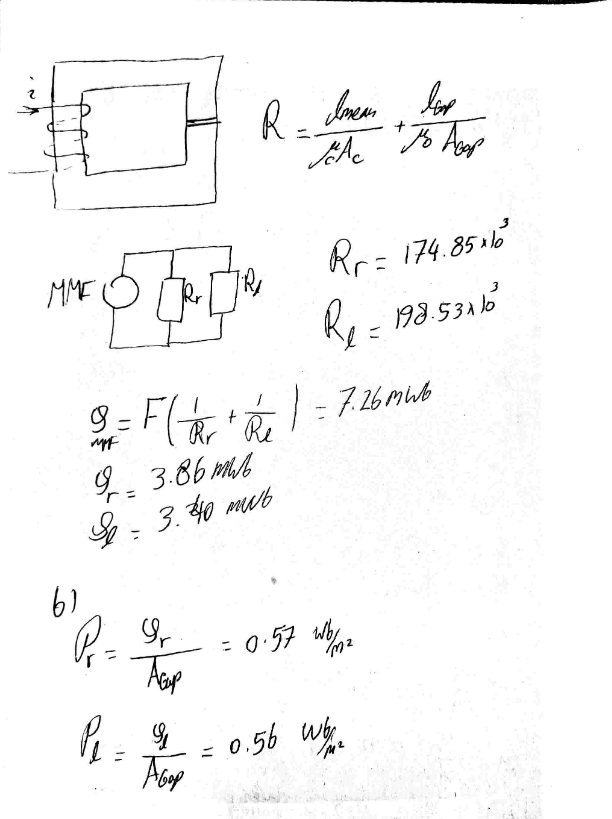
\includegraphics[width = \textwidth]{Prob2.png}
		\end{figure}
		\newpage
		\section{Problem 3}
		We model this problem with a voltage source and a resistor. The magnetic flux is trapped in the core. So, it is constant. 
		The reluctance of the core is obtained by the following equation.
		\begin{equation}
			R = \frac{l_{mean}}{\mu A} = \frac{320}{\mu 400 \, \text{cm}}
		\end{equation} 
		We assume the positive direction of the flux is clockwise.
		\begin{equation}
			F = N_1 i_1 - N_2 i_2 = 28 \, \text{A}
		\end{equation}
		\begin{equation}
			\varphi = \frac{F}{R} = 8.80 \times 10^{-4} \, \text{Wb}
		\end{equation}
		\newpage
		\section{Problem 4}
		\begin{figure}[H]
			\centering
			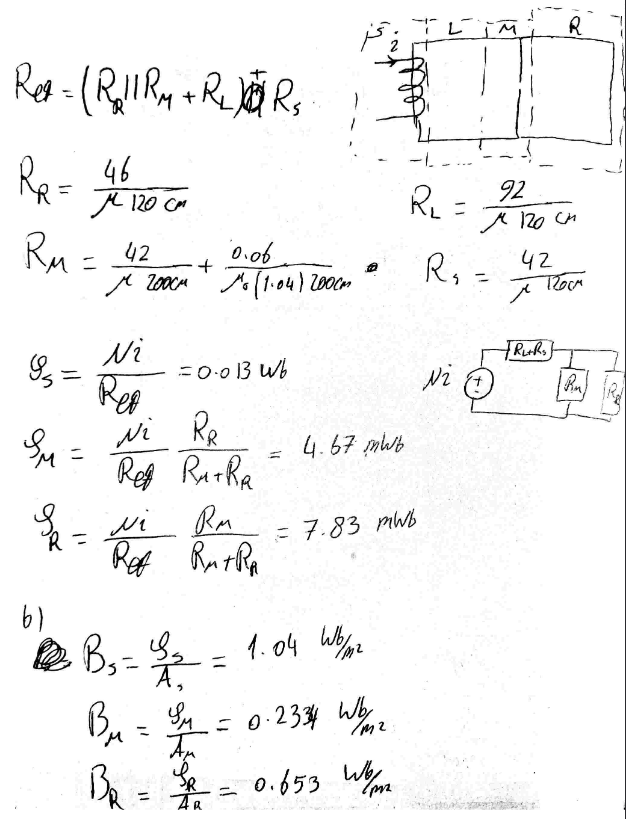
\includegraphics[width = \textwidth]{Prob4.png}
		\end{figure}
		\newpage
		\section{Problem 5}
		In a core(with no branches), magnetic flux is constant. The flux density is almost constant too(a negligible difference in the air gap). But $H$ is not, it is much smaller in the core than the air gap. 
		\begin{equation}
			\int_s \textbf{H}\cdot \text{d}\textbf{l} = N i
		\end{equation}
		\begin{equation}
			H_c l_c + H_a l_a = N i
		\end{equation}
		In the air gap we have $H_a = \frac{B}{\mu_0}$ .Hence,
		\begin{equation}
			H_C(B) l_c + \frac{B}{\mu_0} l_a = N i
		\end{equation}
		We have to find the intersection point of a line and the curve.
		\begin{equation}
			B \approx = 0.47 \, T\quad \to \quad  H_a = 374 \times 10^3 
		\end{equation} 
		
		\section{Problem 6}
		\subsection{a)}
		As determined before,
		\begin{equation}
			H = \frac{472 \, A}{320 \, cm} = 147.5 \, \text{A} \text{m}^{-1}
		\end{equation}
		\begin{equation}
			B = 0.15 \, \text{Wb}
		\end{equation}
		\subsection{b)}
			\begin{equation}
				\mu_r = \frac{H}{B \mu_0} = 809
			\end{equation}	
		\subsection{c)}	
		It depends on our definition of "\textit{good assumption}". The assumption has 20 percent error and represent a significant deviation. In general, this is considered as a very large error. So, it is better to simply say that \textit{this is not a good assumption}. 
		
		\section{Problem 7}
			
		Nature opposes changing magnetic flux, according to Faraday's Law. Therefore, the induced voltage always opposes the direction of the flux change.
		
		\begin{equation}
			v_{ind} = - N\frac{\text{d}\varphi}{dt}
		\end{equation}
		
		\begin{figure}[H]
			\centering
			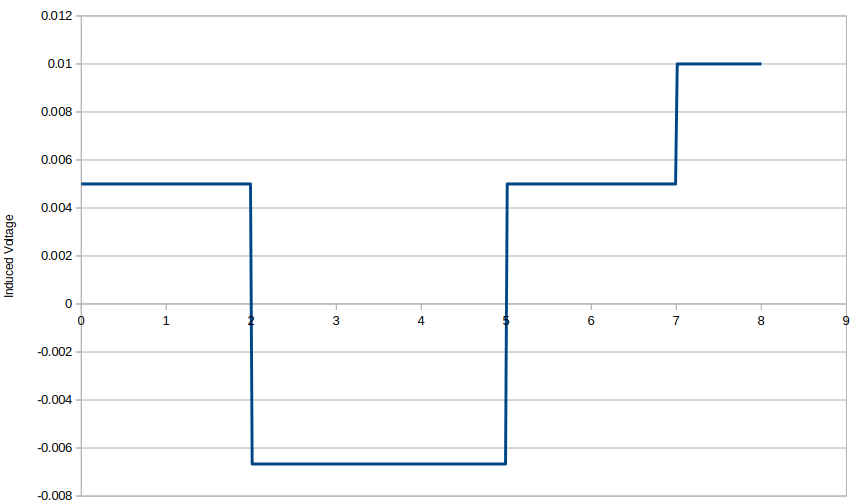
\includegraphics[width = 0.7 \textwidth]{1.png}
			\caption{Induced voltage, Problem 7}
		\end{figure}
		
		\section{Problem 8}
		\subsection{a)}
		Knee point is where the B-H graph starts to flatten out. This is where B has the maximum reasonable value. If the core becomes too saturated, increasing the magnetizing force no longer produces much increase in flux density, making the motor inefficient.
		\begin{equation}
			B\approx 1.3 \, T \quad \& \quad \mu_r = 3300
		\end{equation}
		\subsection{b)}
		\begin{equation}
			\varphi = B_c A_c = 2.08 \times 10^{-3} \, \text{Wb}
		\end{equation}
		\subsection{c)}
		\begin{equation}
			N = \frac{\varphi}{\mu_0 i} \left(\frac{l_c+2R_{rotor}}{\mu_r A_c} + \frac{l_a}{A_a}\right) \approx 1000
		\end{equation}
		\newpage
		\section{Problem 9}
		\begin{figure}[H]
			\centering
			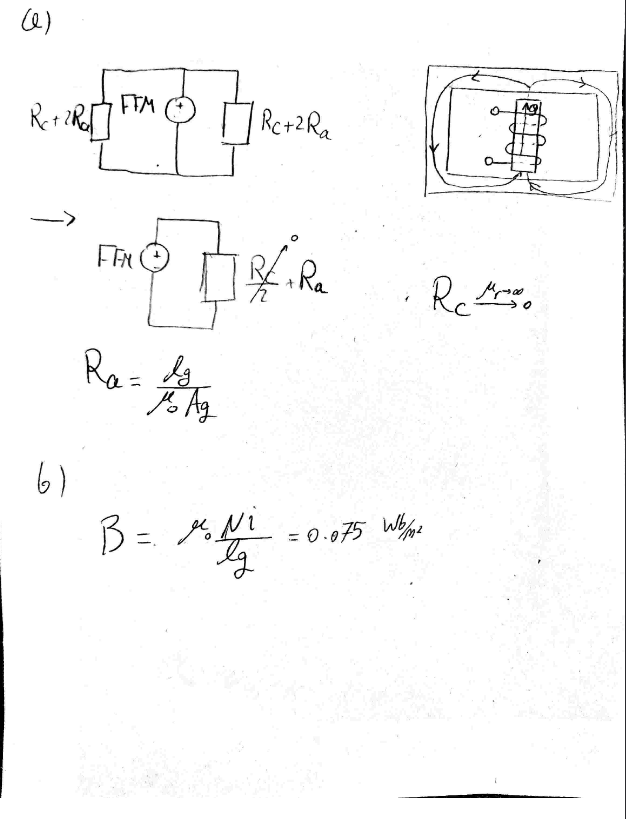
\includegraphics[width = \textwidth]{Prob8.png}
		\end{figure}
		\newpage
		\section{Problem 10}
				\begin{figure}[H]
			\centering
			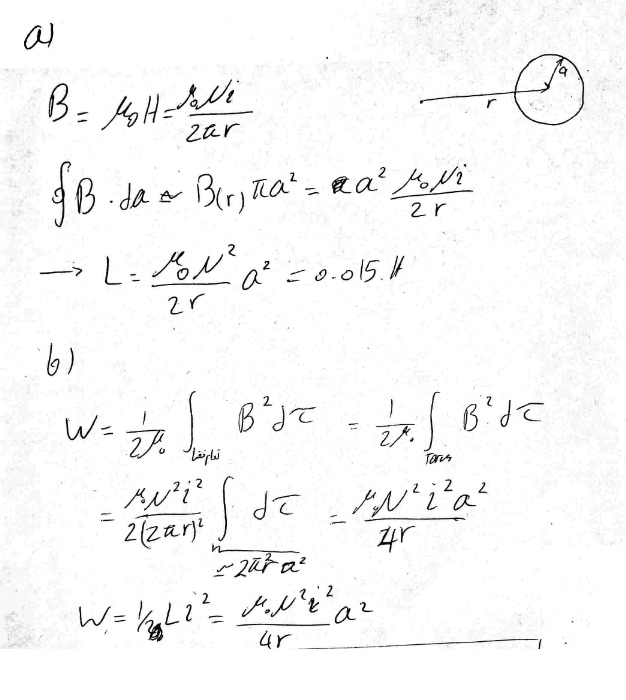
\includegraphics[width = \textwidth]{Prob9-1.png}
		\end{figure}
				\begin{figure}[H]
			\centering
			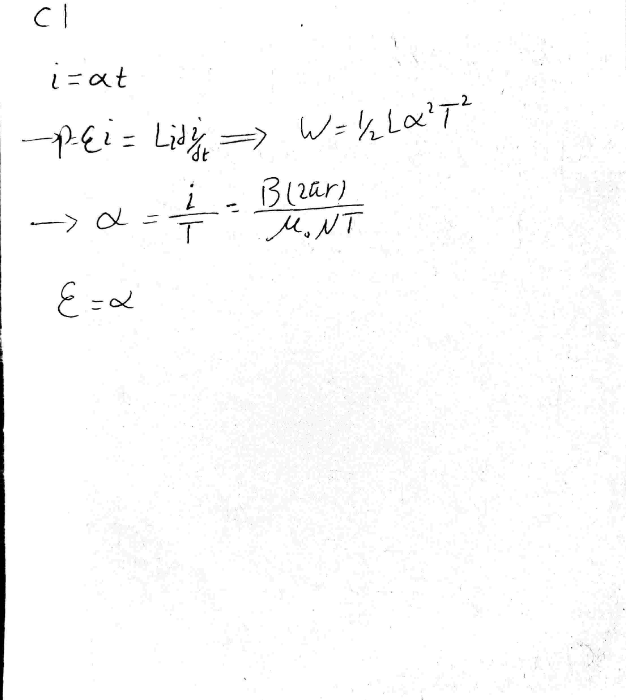
\includegraphics[width = \textwidth]{Prob9-2.png}
		\end{figure}
\end{document}
